\documentclass[twoside]{book}

% Packages required by doxygen
\usepackage{fixltx2e}
\usepackage{calc}
\usepackage{doxygen}
\usepackage[export]{adjustbox} % also loads graphicx
\usepackage{graphicx}
\usepackage[utf8]{inputenc}
\usepackage{makeidx}
\usepackage{multicol}
\usepackage{multirow}
\PassOptionsToPackage{warn}{textcomp}
\usepackage{textcomp}
\usepackage[nointegrals]{wasysym}
\usepackage[table]{xcolor}

% Font selection
\usepackage[T1]{fontenc}
\usepackage[scaled=.90]{helvet}
\usepackage{courier}
\usepackage{amssymb}
\usepackage{sectsty}
\renewcommand{\familydefault}{\sfdefault}
\allsectionsfont{%
  \fontseries{bc}\selectfont%
  \color{darkgray}%
}
\renewcommand{\DoxyLabelFont}{%
  \fontseries{bc}\selectfont%
  \color{darkgray}%
}
\newcommand{\+}{\discretionary{\mbox{\scriptsize$\hookleftarrow$}}{}{}}

% Page & text layout
\usepackage{geometry}
\geometry{%
  a4paper,%
  top=2.5cm,%
  bottom=2.5cm,%
  left=2.5cm,%
  right=2.5cm%
}
\tolerance=750
\hfuzz=15pt
\hbadness=750
\setlength{\emergencystretch}{15pt}
\setlength{\parindent}{0cm}
\setlength{\parskip}{0.2cm}
\makeatletter
\renewcommand{\paragraph}{%
  \@startsection{paragraph}{4}{0ex}{-1.0ex}{1.0ex}{%
    \normalfont\normalsize\bfseries\SS@parafont%
  }%
}
\renewcommand{\subparagraph}{%
  \@startsection{subparagraph}{5}{0ex}{-1.0ex}{1.0ex}{%
    \normalfont\normalsize\bfseries\SS@subparafont%
  }%
}
\makeatother

% Headers & footers
\usepackage{fancyhdr}
\pagestyle{fancyplain}
\fancyhead[LE]{\fancyplain{}{\bfseries\thepage}}
\fancyhead[CE]{\fancyplain{}{}}
\fancyhead[RE]{\fancyplain{}{\bfseries\leftmark}}
\fancyhead[LO]{\fancyplain{}{\bfseries\rightmark}}
\fancyhead[CO]{\fancyplain{}{}}
\fancyhead[RO]{\fancyplain{}{\bfseries\thepage}}
\fancyfoot[LE]{\fancyplain{}{}}
\fancyfoot[CE]{\fancyplain{}{}}
\fancyfoot[RE]{\fancyplain{}{\bfseries\scriptsize Generated on Wed Sep 9 2015 17\+:40\+:01 for Pyagilis by Doxygen }}
\fancyfoot[LO]{\fancyplain{}{\bfseries\scriptsize Generated on Wed Sep 9 2015 17\+:40\+:01 for Pyagilis by Doxygen }}
\fancyfoot[CO]{\fancyplain{}{}}
\fancyfoot[RO]{\fancyplain{}{}}
\renewcommand{\footrulewidth}{0.4pt}
\renewcommand{\chaptermark}[1]{%
  \markboth{#1}{}%
}
\renewcommand{\sectionmark}[1]{%
  \markright{\thesection\ #1}%
}

% Indices & bibliography
\usepackage{natbib}
\usepackage[titles]{tocloft}
\setcounter{tocdepth}{3}
\setcounter{secnumdepth}{5}
\makeindex

% Hyperlinks (required, but should be loaded last)
\usepackage{ifpdf}
\ifpdf
  \usepackage[pdftex,pagebackref=true]{hyperref}
\else
  \usepackage[ps2pdf,pagebackref=true]{hyperref}
\fi
\hypersetup{%
  colorlinks=true,%
  linkcolor=blue,%
  citecolor=blue,%
  unicode%
}

% Custom commands
\newcommand{\clearemptydoublepage}{%
  \newpage{\pagestyle{empty}\cleardoublepage}%
}


%===== C O N T E N T S =====

\begin{document}

% Titlepage & ToC
\hypersetup{pageanchor=false,
             bookmarks=true,
             bookmarksnumbered=true,
             pdfencoding=unicode
            }
\pagenumbering{roman}
\begin{titlepage}
\vspace*{7cm}
\begin{center}%
{\Large Pyagilis }\\
\vspace*{1cm}
{\large Generated by Doxygen 1.8.10}\\
\vspace*{0.5cm}
{\small Wed Sep 9 2015 17:40:01}\\
\end{center}
\end{titlepage}
\clearemptydoublepage
\tableofcontents
\clearemptydoublepage
\pagenumbering{arabic}
\hypersetup{pageanchor=true}

%--- Begin generated contents ---
\chapter{pyagilis}
\label{md__r_e_a_d_m_e}
\hypertarget{md__r_e_a_d_m_e}{}
This is a python library for Newport Agilis piezo motion controllers (\href{https://www.newport.com/Agilis-Piezo-Motion-Controllers/848283/1033/info.aspx}{\tt https\+://www.\+newport.\+com/\+Agilis-\/\+Piezo-\/\+Motion-\/\+Controllers/848283/1033/info.\+aspx}) 
\chapter{Namespace Index}
\section{Namespace List}
Here is a list of all documented namespaces with brief descriptions\+:\begin{DoxyCompactList}
\item\contentsline{section}{\hyperlink{namespaceag_port}{ag\+Port} \\*This module contain classes that implements custom versions of python built-\/in serial port class for the agilis controllers }{\pageref{namespaceag_port}}{}
\end{DoxyCompactList}

\chapter{Hierarchical Index}
\section{Class Hierarchy}
This inheritance list is sorted roughly, but not completely, alphabetically\+:\begin{DoxyCompactList}
\item object\begin{DoxyCompactList}
\item \contentsline{section}{pyagilis.\+channel.\+Axis}{\pageref{classpyagilis_1_1channel_1_1_axis}}{}
\item \contentsline{section}{pyagilis.\+controller.\+A\+G\+U\+C2}{\pageref{classpyagilis_1_1controller_1_1_a_g_u_c2}}{}
\item \contentsline{section}{pyagilis.\+controller.\+A\+G\+U\+C8}{\pageref{classpyagilis_1_1controller_1_1_a_g_u_c8}}{}
\end{DoxyCompactList}
\item Serial\begin{DoxyCompactList}
\item \contentsline{section}{pyagilis.\+ag\+Port.\+A\+G\+Port}{\pageref{classpyagilis_1_1ag_port_1_1_a_g_port}}{}
\end{DoxyCompactList}
\item Thread\begin{DoxyCompactList}
\item \contentsline{section}{pyagilis.\+mothreading.\+Motor\+Thread}{\pageref{classpyagilis_1_1mothreading_1_1_motor_thread}}{}
\end{DoxyCompactList}
\end{DoxyCompactList}

\chapter{Class Index}
\section{Class List}
Here are the classes, structs, unions and interfaces with brief descriptions\+:\begin{DoxyCompactList}
\item\contentsline{section}{\hyperlink{classpyagilis_1_1ag_port_1_1_a_g_port}{pyagilis.\+ag\+Port.\+A\+G\+Port} \\*Documentatio for the \hyperlink{classpyagilis_1_1ag_port_1_1_a_g_port}{A\+G\+Port} class }{\pageref{classpyagilis_1_1ag_port_1_1_a_g_port}}{}
\item\contentsline{section}{\hyperlink{classpyagilis_1_1controller_1_1_a_g_u_c2}{pyagilis.\+controller.\+A\+G\+U\+C2} }{\pageref{classpyagilis_1_1controller_1_1_a_g_u_c2}}{}
\item\contentsline{section}{\hyperlink{classpyagilis_1_1controller_1_1_a_g_u_c8}{pyagilis.\+controller.\+A\+G\+U\+C8} }{\pageref{classpyagilis_1_1controller_1_1_a_g_u_c8}}{}
\item\contentsline{section}{\hyperlink{classpyagilis_1_1channel_1_1_axis}{pyagilis.\+channel.\+Axis} }{\pageref{classpyagilis_1_1channel_1_1_axis}}{}
\item\contentsline{section}{\hyperlink{classpyagilis_1_1mothreading_1_1_motor_thread}{pyagilis.\+mothreading.\+Motor\+Thread} }{\pageref{classpyagilis_1_1mothreading_1_1_motor_thread}}{}
\end{DoxyCompactList}

\chapter{Namespace Documentation}
\hypertarget{namespaceag_port}{}\section{ag\+Port Namespace Reference}
\label{namespaceag_port}\index{ag\+Port@{ag\+Port}}


This module contain classes that implements custom versions of python built-\/in serial port class for the agilis controllers.  




\subsection{Detailed Description}
This module contain classes that implements custom versions of python built-\/in serial port class for the agilis controllers. 
\chapter{Class Documentation}
\hypertarget{classpyagilis_1_1ag_port_1_1_a_g_port}{}\section{pyagilis.\+ag\+Port.\+A\+G\+Port Class Reference}
\label{classpyagilis_1_1ag_port_1_1_a_g_port}\index{pyagilis.\+ag\+Port.\+A\+G\+Port@{pyagilis.\+ag\+Port.\+A\+G\+Port}}


Documentatio for the \hyperlink{classpyagilis_1_1ag_port_1_1_a_g_port}{A\+G\+Port} class.  


Inheritance diagram for pyagilis.\+ag\+Port.\+A\+G\+Port\+:\begin{figure}[H]
\begin{center}
\leavevmode
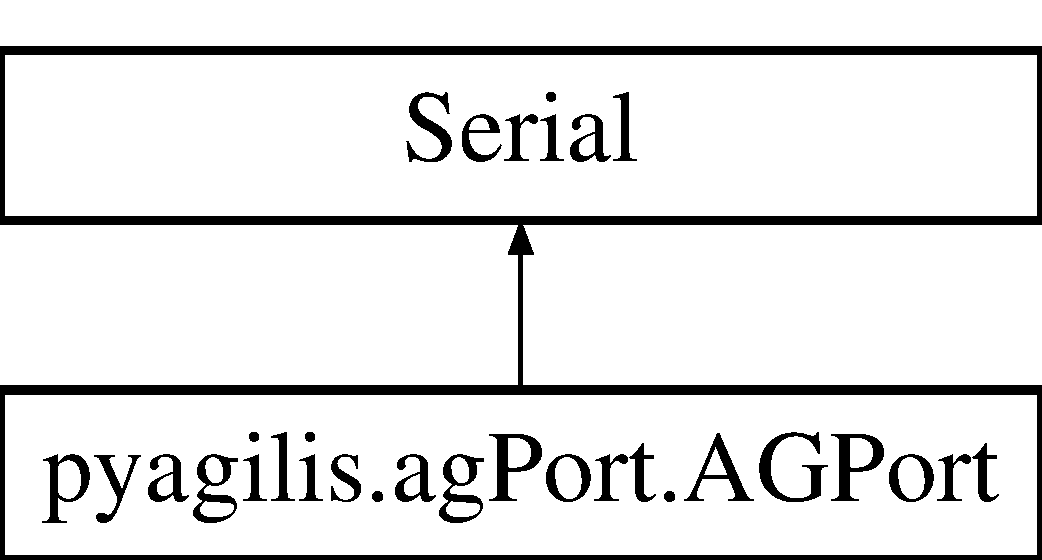
\includegraphics[height=2.000000cm]{classpyagilis_1_1ag_port_1_1_a_g_port}
\end{center}
\end{figure}
\subsection*{Public Member Functions}
\begin{DoxyCompactItemize}
\item 
def \hyperlink{classpyagilis_1_1ag_port_1_1_a_g_port_a82b3f965764f6ddbef5ebcc89e908f54}{\+\_\+\+\_\+init\+\_\+\+\_\+}
\begin{DoxyCompactList}\small\item\em Class constructor. \end{DoxyCompactList}\item 
\hypertarget{classpyagilis_1_1ag_port_1_1_a_g_port_ad854d770b84316549e659f7df1d06774}{}def {\bfseries am\+Inull} (self)\label{classpyagilis_1_1ag_port_1_1_a_g_port_ad854d770b84316549e659f7df1d06774}

\item 
\hypertarget{classpyagilis_1_1ag_port_1_1_a_g_port_ac953c8cc75fe959e4a34729cbd812509}{}def {\bfseries is\+Aquery} (self, command)\label{classpyagilis_1_1ag_port_1_1_a_g_port_ac953c8cc75fe959e4a34729cbd812509}

\item 
\hypertarget{classpyagilis_1_1ag_port_1_1_a_g_port_a819b6127c2b4eb7aaa16b51d49f51542}{}def {\bfseries send\+String} (self, command)\label{classpyagilis_1_1ag_port_1_1_a_g_port_a819b6127c2b4eb7aaa16b51d49f51542}

\end{DoxyCompactItemize}
\subsection*{Public Attributes}
\begin{DoxyCompactItemize}
\item 
\hypertarget{classpyagilis_1_1ag_port_1_1_a_g_port_ae3be10cf10588bc548ab78fba704779e}{}{\bfseries soul}\label{classpyagilis_1_1ag_port_1_1_a_g_port_ae3be10cf10588bc548ab78fba704779e}

\end{DoxyCompactItemize}


\subsection{Detailed Description}
Documentatio for the \hyperlink{classpyagilis_1_1ag_port_1_1_a_g_port}{A\+G\+Port} class. 

This class extend the python Serial class with some function that simplifies its use with the agilis controllers commands 

\subsection{Constructor \& Destructor Documentation}
\hypertarget{classpyagilis_1_1ag_port_1_1_a_g_port_a82b3f965764f6ddbef5ebcc89e908f54}{}\index{pyagilis\+::ag\+Port\+::\+A\+G\+Port@{pyagilis\+::ag\+Port\+::\+A\+G\+Port}!\+\_\+\+\_\+init\+\_\+\+\_\+@{\+\_\+\+\_\+init\+\_\+\+\_\+}}
\index{\+\_\+\+\_\+init\+\_\+\+\_\+@{\+\_\+\+\_\+init\+\_\+\+\_\+}!pyagilis\+::ag\+Port\+::\+A\+G\+Port@{pyagilis\+::ag\+Port\+::\+A\+G\+Port}}
\subsubsection[{\+\_\+\+\_\+init\+\_\+\+\_\+}]{\setlength{\rightskip}{0pt plus 5cm}def pyagilis.\+ag\+Port.\+A\+G\+Port.\+\_\+\+\_\+init\+\_\+\+\_\+ (
\begin{DoxyParamCaption}
\item[{}]{self, }
\item[{}]{port\+Name = {\ttfamily None}}
\end{DoxyParamCaption}
)}\label{classpyagilis_1_1ag_port_1_1_a_g_port_a82b3f965764f6ddbef5ebcc89e908f54}


Class constructor. 


\begin{DoxyParams}{Parameters}
{\em port\+Name} & The name of the virtual serial port of the chosen controller \\
\hline
\end{DoxyParams}


The documentation for this class was generated from the following file\+:\begin{DoxyCompactItemize}
\item 
ag\+Port.\+py\end{DoxyCompactItemize}

\hypertarget{classpyagilis_1_1controller_1_1_a_g_u_c2}{}\section{pyagilis.\+controller.\+A\+G\+U\+C2 Class Reference}
\label{classpyagilis_1_1controller_1_1_a_g_u_c2}\index{pyagilis.\+controller.\+A\+G\+U\+C2@{pyagilis.\+controller.\+A\+G\+U\+C2}}
Inheritance diagram for pyagilis.\+controller.\+A\+G\+U\+C2\+:\begin{figure}[H]
\begin{center}
\leavevmode
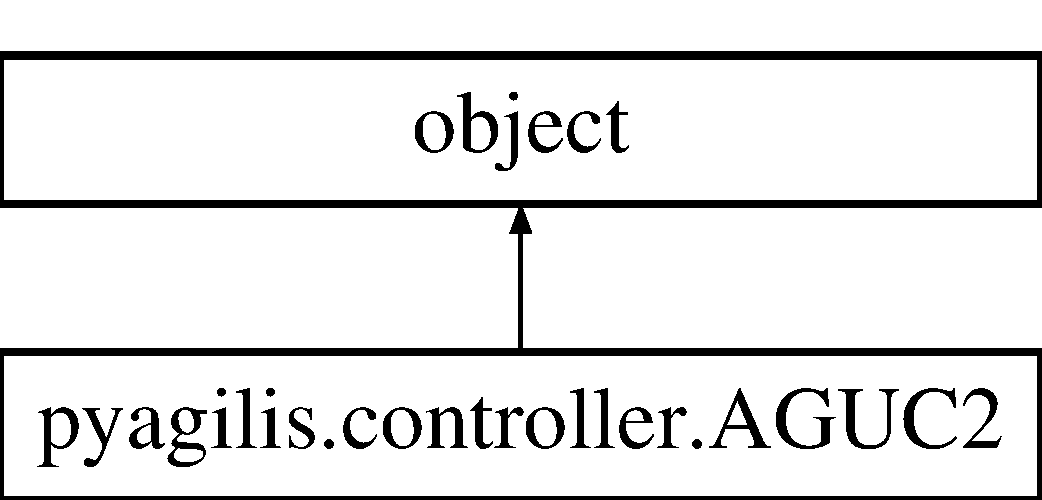
\includegraphics[height=2.000000cm]{classpyagilis_1_1controller_1_1_a_g_u_c2}
\end{center}
\end{figure}
\subsection*{Public Member Functions}
\begin{DoxyCompactItemize}
\item 
\hypertarget{classpyagilis_1_1controller_1_1_a_g_u_c2_ab656159b6f37bc8ea9cf9c7751997f7a}{}def {\bfseries \+\_\+\+\_\+init\+\_\+\+\_\+}\label{classpyagilis_1_1controller_1_1_a_g_u_c2_ab656159b6f37bc8ea9cf9c7751997f7a}

\item 
\hypertarget{classpyagilis_1_1controller_1_1_a_g_u_c2_a5e26c9c3aa2aab927c80694b8b6589f2}{}def {\bfseries add\+Axis} (self, name, alias, step\+Amp)\label{classpyagilis_1_1controller_1_1_a_g_u_c2_a5e26c9c3aa2aab927c80694b8b6589f2}

\item 
\hypertarget{classpyagilis_1_1controller_1_1_a_g_u_c2_a58689649d666054fe1cf7de33dbabf18}{}def {\bfseries move} (self, d1, d2)\label{classpyagilis_1_1controller_1_1_a_g_u_c2_a58689649d666054fe1cf7de33dbabf18}

\item 
\hypertarget{classpyagilis_1_1controller_1_1_a_g_u_c2_aad7546b56a68f8e8fc21a382f856f683}{}def {\bfseries move\+Up\+Up} (self)\label{classpyagilis_1_1controller_1_1_a_g_u_c2_aad7546b56a68f8e8fc21a382f856f683}

\item 
\hypertarget{classpyagilis_1_1controller_1_1_a_g_u_c2_a40012f646cef7df7782228c8f38e2fa6}{}def {\bfseries move\+Down\+Down} (self)\label{classpyagilis_1_1controller_1_1_a_g_u_c2_a40012f646cef7df7782228c8f38e2fa6}

\item 
\hypertarget{classpyagilis_1_1controller_1_1_a_g_u_c2_ac33686581cb371f1f28f85ac0885feba}{}def {\bfseries move\+Down\+Up} (self)\label{classpyagilis_1_1controller_1_1_a_g_u_c2_ac33686581cb371f1f28f85ac0885feba}

\item 
\hypertarget{classpyagilis_1_1controller_1_1_a_g_u_c2_a6d6c49207444187959d3f3afaca3c73f}{}def {\bfseries move\+Up\+Down} (self)\label{classpyagilis_1_1controller_1_1_a_g_u_c2_a6d6c49207444187959d3f3afaca3c73f}

\item 
\hypertarget{classpyagilis_1_1controller_1_1_a_g_u_c2_ae3426367a5605c19e779773e59f58de9}{}def {\bfseries go\+To\+Zero} (self)\label{classpyagilis_1_1controller_1_1_a_g_u_c2_ae3426367a5605c19e779773e59f58de9}

\item 
\hypertarget{classpyagilis_1_1controller_1_1_a_g_u_c2_a33b44b25a249e4b84690f6d419015170}{}def {\bfseries set\+Zero} (self)\label{classpyagilis_1_1controller_1_1_a_g_u_c2_a33b44b25a249e4b84690f6d419015170}

\item 
\hypertarget{classpyagilis_1_1controller_1_1_a_g_u_c2_aa477fada704e720021125f4cd90a246d}{}def {\bfseries stop} (self)\label{classpyagilis_1_1controller_1_1_a_g_u_c2_aa477fada704e720021125f4cd90a246d}

\item 
\hypertarget{classpyagilis_1_1controller_1_1_a_g_u_c2_a4e33dbd5194d82d17375a7353bbd3eab}{}def {\bfseries follow\+Apath} (self, path)\label{classpyagilis_1_1controller_1_1_a_g_u_c2_a4e33dbd5194d82d17375a7353bbd3eab}

\end{DoxyCompactItemize}
\subsection*{Public Attributes}
\begin{DoxyCompactItemize}
\item 
\hypertarget{classpyagilis_1_1controller_1_1_a_g_u_c2_ad83a76829f65a17b43d2d50167a170d9}{}{\bfseries port}\label{classpyagilis_1_1controller_1_1_a_g_u_c2_ad83a76829f65a17b43d2d50167a170d9}

\item 
\hypertarget{classpyagilis_1_1controller_1_1_a_g_u_c2_ac56df0be4d47a97c893330a5a332a738}{}{\bfseries axis}\label{classpyagilis_1_1controller_1_1_a_g_u_c2_ac56df0be4d47a97c893330a5a332a738}

\item 
\hypertarget{classpyagilis_1_1controller_1_1_a_g_u_c2_aca4825e154ba7c1d0983fe450086377c}{}{\bfseries aliases}\label{classpyagilis_1_1controller_1_1_a_g_u_c2_aca4825e154ba7c1d0983fe450086377c}

\item 
\hypertarget{classpyagilis_1_1controller_1_1_a_g_u_c2_ac45fee51f82e78301a27eee0f1adc3dd}{}{\bfseries m\+Thread}\label{classpyagilis_1_1controller_1_1_a_g_u_c2_ac45fee51f82e78301a27eee0f1adc3dd}

\end{DoxyCompactItemize}


The documentation for this class was generated from the following file\+:\begin{DoxyCompactItemize}
\item 
controller.\+py\end{DoxyCompactItemize}

\hypertarget{classpyagilis_1_1controller_1_1_a_g_u_c8}{}\section{pyagilis.\+controller.\+A\+G\+U\+C8 Class Reference}
\label{classpyagilis_1_1controller_1_1_a_g_u_c8}\index{pyagilis.\+controller.\+A\+G\+U\+C8@{pyagilis.\+controller.\+A\+G\+U\+C8}}
Inheritance diagram for pyagilis.\+controller.\+A\+G\+U\+C8\+:\begin{figure}[H]
\begin{center}
\leavevmode
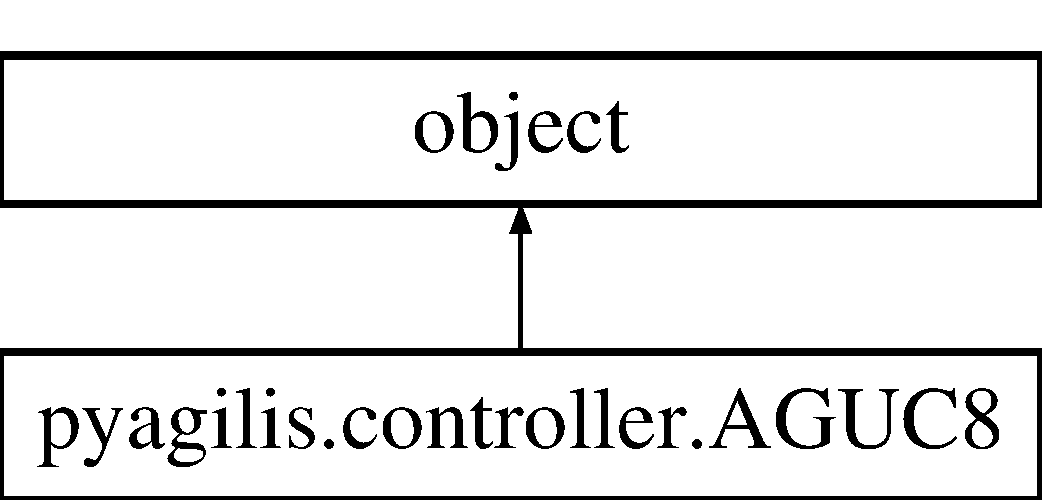
\includegraphics[height=2.000000cm]{classpyagilis_1_1controller_1_1_a_g_u_c8}
\end{center}
\end{figure}
\subsection*{Public Member Functions}
\begin{DoxyCompactItemize}
\item 
\hypertarget{classpyagilis_1_1controller_1_1_a_g_u_c8_a9bc6969227da436d24fca3081860f438}{}def {\bfseries \+\_\+\+\_\+init\+\_\+\+\_\+}\label{classpyagilis_1_1controller_1_1_a_g_u_c8_a9bc6969227da436d24fca3081860f438}

\item 
\hypertarget{classpyagilis_1_1controller_1_1_a_g_u_c8_a4c7e1b52f93d89332d80da5ca8bde688}{}def {\bfseries chchch} (self, ch)\label{classpyagilis_1_1controller_1_1_a_g_u_c8_a4c7e1b52f93d89332d80da5ca8bde688}

\item 
\hypertarget{classpyagilis_1_1controller_1_1_a_g_u_c8_aec0759230e82111cb87e9a74708d2520}{}def {\bfseries add\+Axis} (self, channel, name, alias, step\+Amp)\label{classpyagilis_1_1controller_1_1_a_g_u_c8_aec0759230e82111cb87e9a74708d2520}

\item 
\hypertarget{classpyagilis_1_1controller_1_1_a_g_u_c8_ade6d12edb331d328af5eac095b46a0ae}{}def {\bfseries move} (self, ch, d1, d2)\label{classpyagilis_1_1controller_1_1_a_g_u_c8_ade6d12edb331d328af5eac095b46a0ae}

\item 
\hypertarget{classpyagilis_1_1controller_1_1_a_g_u_c8_a88bc6a3a60de40486b69867d0c596472}{}def {\bfseries move\+Up\+Up} (self, ch)\label{classpyagilis_1_1controller_1_1_a_g_u_c8_a88bc6a3a60de40486b69867d0c596472}

\item 
\hypertarget{classpyagilis_1_1controller_1_1_a_g_u_c8_ae8f4fada82520979b46d8a862e759707}{}def {\bfseries move\+Down\+Down} (self, ch)\label{classpyagilis_1_1controller_1_1_a_g_u_c8_ae8f4fada82520979b46d8a862e759707}

\item 
\hypertarget{classpyagilis_1_1controller_1_1_a_g_u_c8_a3d00f6a96a740cd7181281c07c2b1ccf}{}def {\bfseries move\+Down\+Up} (self, ch)\label{classpyagilis_1_1controller_1_1_a_g_u_c8_a3d00f6a96a740cd7181281c07c2b1ccf}

\item 
\hypertarget{classpyagilis_1_1controller_1_1_a_g_u_c8_acde9b9adfded39a6f28e1b8a48a58e84}{}def {\bfseries move\+Up\+Down} (self, ch)\label{classpyagilis_1_1controller_1_1_a_g_u_c8_acde9b9adfded39a6f28e1b8a48a58e84}

\item 
\hypertarget{classpyagilis_1_1controller_1_1_a_g_u_c8_ac6a1b091b8351096db6abd5d9aa09a42}{}def {\bfseries go\+To\+Zero} (self, ch)\label{classpyagilis_1_1controller_1_1_a_g_u_c8_ac6a1b091b8351096db6abd5d9aa09a42}

\item 
\hypertarget{classpyagilis_1_1controller_1_1_a_g_u_c8_a792b3c9ce6d0365b65d1bf75acf9c179}{}def {\bfseries set\+Zero} (self, ch)\label{classpyagilis_1_1controller_1_1_a_g_u_c8_a792b3c9ce6d0365b65d1bf75acf9c179}

\item 
\hypertarget{classpyagilis_1_1controller_1_1_a_g_u_c8_af8908bdd36660efbf728cf9e216ae283}{}def {\bfseries stop} (self, ch)\label{classpyagilis_1_1controller_1_1_a_g_u_c8_af8908bdd36660efbf728cf9e216ae283}

\item 
\hypertarget{classpyagilis_1_1controller_1_1_a_g_u_c8_aba2c96a77f17f21613d07f152abee0a3}{}def {\bfseries follow\+Apath} (self, ch, path)\label{classpyagilis_1_1controller_1_1_a_g_u_c8_aba2c96a77f17f21613d07f152abee0a3}

\end{DoxyCompactItemize}
\subsection*{Public Attributes}
\begin{DoxyCompactItemize}
\item 
\hypertarget{classpyagilis_1_1controller_1_1_a_g_u_c8_a1fbc03520bbc818fa6b7068c2d18082c}{}{\bfseries port}\label{classpyagilis_1_1controller_1_1_a_g_u_c8_a1fbc03520bbc818fa6b7068c2d18082c}

\item 
\hypertarget{classpyagilis_1_1controller_1_1_a_g_u_c8_a0e10ce1697aba8e72640dfcb70a20676}{}{\bfseries channels}\label{classpyagilis_1_1controller_1_1_a_g_u_c8_a0e10ce1697aba8e72640dfcb70a20676}

\item 
\hypertarget{classpyagilis_1_1controller_1_1_a_g_u_c8_a808be674a6d2dd0227d90260b8e84c5a}{}{\bfseries aliases}\label{classpyagilis_1_1controller_1_1_a_g_u_c8_a808be674a6d2dd0227d90260b8e84c5a}

\item 
\hypertarget{classpyagilis_1_1controller_1_1_a_g_u_c8_ab8f488a1f3eb3142d82a38ff8c4303e4}{}{\bfseries m\+Thread}\label{classpyagilis_1_1controller_1_1_a_g_u_c8_ab8f488a1f3eb3142d82a38ff8c4303e4}

\end{DoxyCompactItemize}


The documentation for this class was generated from the following file\+:\begin{DoxyCompactItemize}
\item 
controller.\+py\end{DoxyCompactItemize}

\hypertarget{classpyagilis_1_1channel_1_1_axis}{}\section{pyagilis.\+channel.\+Axis Class Reference}
\label{classpyagilis_1_1channel_1_1_axis}\index{pyagilis.\+channel.\+Axis@{pyagilis.\+channel.\+Axis}}
Inheritance diagram for pyagilis.\+channel.\+Axis\+:\begin{figure}[H]
\begin{center}
\leavevmode
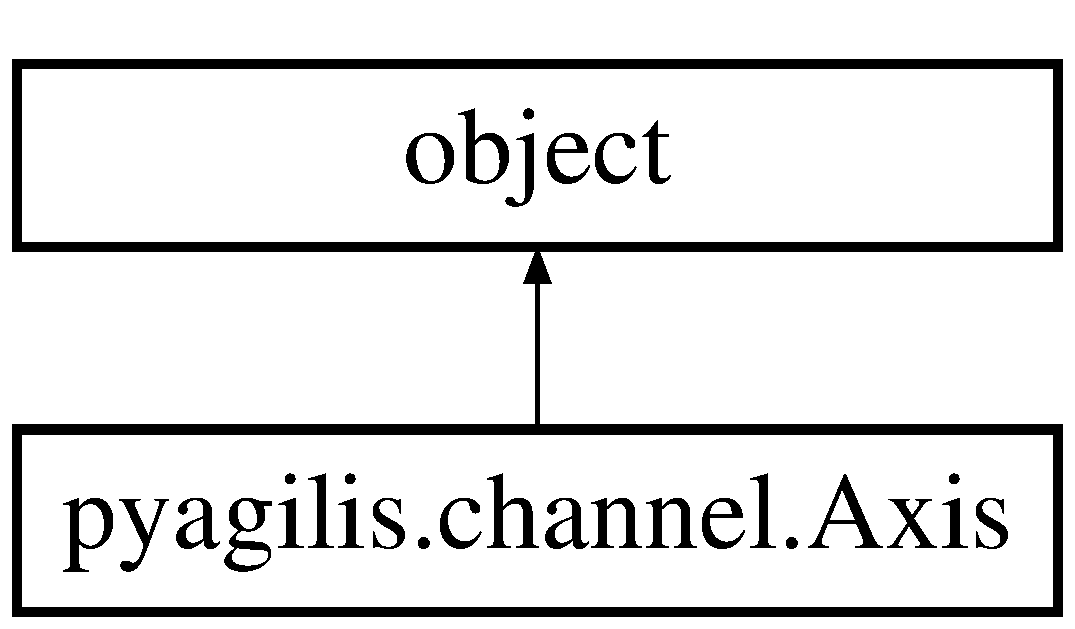
\includegraphics[height=2.000000cm]{classpyagilis_1_1channel_1_1_axis}
\end{center}
\end{figure}
\subsection*{Public Member Functions}
\begin{DoxyCompactItemize}
\item 
\hypertarget{classpyagilis_1_1channel_1_1_axis_af8ecbb92dc3dcf8dd10dd28bb32c6a70}{}def {\bfseries \+\_\+\+\_\+init\+\_\+\+\_\+}\label{classpyagilis_1_1channel_1_1_axis_af8ecbb92dc3dcf8dd10dd28bb32c6a70}

\item 
\hypertarget{classpyagilis_1_1channel_1_1_axis_ab458b724a8a556c1eda5e59e0a039864}{}def {\bfseries what\+Did\+Ido} (self)\label{classpyagilis_1_1channel_1_1_axis_ab458b724a8a556c1eda5e59e0a039864}

\item 
\hypertarget{classpyagilis_1_1channel_1_1_axis_a0687290da2151921e70a9b888286b1ba}{}def {\bfseries stop} (self)\label{classpyagilis_1_1channel_1_1_axis_a0687290da2151921e70a9b888286b1ba}

\item 
\hypertarget{classpyagilis_1_1channel_1_1_axis_a3db253c98e023dc3aa3dc5e4cb22c019}{}def {\bfseries am\+Istill} (self, rate)\label{classpyagilis_1_1channel_1_1_axis_a3db253c98e023dc3aa3dc5e4cb22c019}

\item 
\hypertarget{classpyagilis_1_1channel_1_1_axis_a9c33e5258d04f1669fb91c726ee1388e}{}def {\bfseries am\+Iat\+My\+Limit} (self)\label{classpyagilis_1_1channel_1_1_axis_a9c33e5258d04f1669fb91c726ee1388e}

\item 
\hypertarget{classpyagilis_1_1channel_1_1_axis_a738f87c70fdea3a66009b44da15ed2a0}{}def {\bfseries query\+Counter} (self)\label{classpyagilis_1_1channel_1_1_axis_a738f87c70fdea3a66009b44da15ed2a0}

\item 
\hypertarget{classpyagilis_1_1channel_1_1_axis_a4303e1496baae0c2689b1d3df23ddbfa}{}def {\bfseries reset\+Counter} (self)\label{classpyagilis_1_1channel_1_1_axis_a4303e1496baae0c2689b1d3df23ddbfa}

\item 
\hypertarget{classpyagilis_1_1channel_1_1_axis_adb3f82948d9d2cabf475a315885742d1}{}def {\bfseries jog}\label{classpyagilis_1_1channel_1_1_axis_adb3f82948d9d2cabf475a315885742d1}

\item 
\hypertarget{classpyagilis_1_1channel_1_1_axis_abe9ced6fe87bb3494369a7f017097442}{}def {\bfseries go\+Max}\label{classpyagilis_1_1channel_1_1_axis_abe9ced6fe87bb3494369a7f017097442}

\item 
\hypertarget{classpyagilis_1_1channel_1_1_axis_a87ae68b64bf7fa461771332a816881c3}{}def {\bfseries go\+Min}\label{classpyagilis_1_1channel_1_1_axis_a87ae68b64bf7fa461771332a816881c3}

\item 
\hypertarget{classpyagilis_1_1channel_1_1_axis_a35b891433b2442ecc6dfea5173afc474}{}def {\bfseries now\+To\+Milliseconds} (self)\label{classpyagilis_1_1channel_1_1_axis_a35b891433b2442ecc6dfea5173afc474}

\item 
\hypertarget{classpyagilis_1_1channel_1_1_axis_a64b33a63785163690ef6cb614cf82d89}{}def {\bfseries wait\+Me} (self, interval)\label{classpyagilis_1_1channel_1_1_axis_a64b33a63785163690ef6cb614cf82d89}

\end{DoxyCompactItemize}
\subsection*{Public Attributes}
\begin{DoxyCompactItemize}
\item 
\hypertarget{classpyagilis_1_1channel_1_1_axis_a1012600214e52116d1ffeb867e31bc71}{}{\bfseries controller}\label{classpyagilis_1_1channel_1_1_axis_a1012600214e52116d1ffeb867e31bc71}

\item 
\hypertarget{classpyagilis_1_1channel_1_1_axis_a8f5e7062a84a856b6da6caf72e4b009a}{}{\bfseries name}\label{classpyagilis_1_1channel_1_1_axis_a8f5e7062a84a856b6da6caf72e4b009a}

\item 
\hypertarget{classpyagilis_1_1channel_1_1_axis_a1a7fae27a7e1c59866900893c4f38e54}{}{\bfseries rate}\label{classpyagilis_1_1channel_1_1_axis_a1a7fae27a7e1c59866900893c4f38e54}

\item 
\hypertarget{classpyagilis_1_1channel_1_1_axis_af1661ca84757249d14c3b8275e4a01c9}{}{\bfseries step\+Amp}\label{classpyagilis_1_1channel_1_1_axis_af1661ca84757249d14c3b8275e4a01c9}

\end{DoxyCompactItemize}


The documentation for this class was generated from the following file\+:\begin{DoxyCompactItemize}
\item 
channel.\+py\end{DoxyCompactItemize}

\hypertarget{classpyagilis_1_1mothreading_1_1_motor_thread}{}\section{pyagilis.\+mothreading.\+Motor\+Thread Class Reference}
\label{classpyagilis_1_1mothreading_1_1_motor_thread}\index{pyagilis.\+mothreading.\+Motor\+Thread@{pyagilis.\+mothreading.\+Motor\+Thread}}
Inheritance diagram for pyagilis.\+mothreading.\+Motor\+Thread\+:\begin{figure}[H]
\begin{center}
\leavevmode
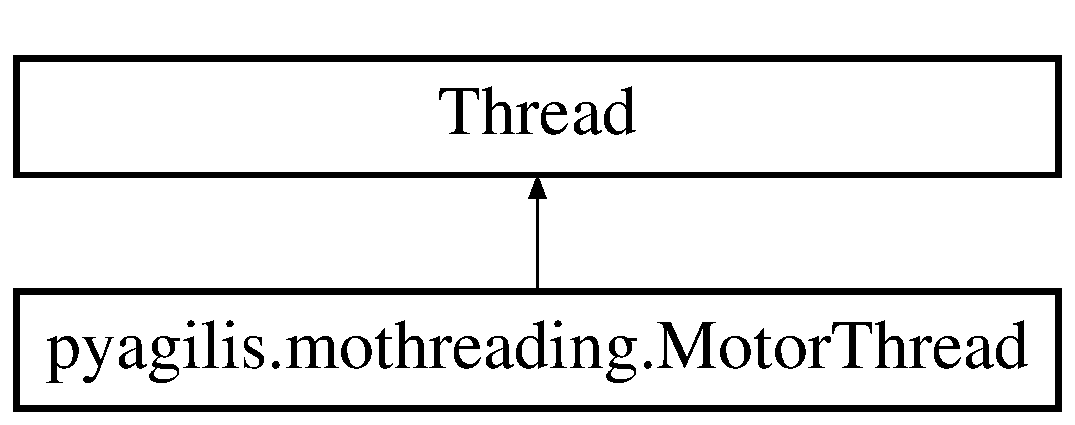
\includegraphics[height=2.000000cm]{classpyagilis_1_1mothreading_1_1_motor_thread}
\end{center}
\end{figure}
\subsection*{Public Member Functions}
\begin{DoxyCompactItemize}
\item 
\hypertarget{classpyagilis_1_1mothreading_1_1_motor_thread_a48ac0fde5f66cbf50b74ad97ebf2403f}{}def {\bfseries \+\_\+\+\_\+init\+\_\+\+\_\+}\label{classpyagilis_1_1mothreading_1_1_motor_thread_a48ac0fde5f66cbf50b74ad97ebf2403f}

\item 
\hypertarget{classpyagilis_1_1mothreading_1_1_motor_thread_a4a51f3fdb44af60ad64fa8e22e0f78ba}{}def {\bfseries exec\+Step} (self, step)\label{classpyagilis_1_1mothreading_1_1_motor_thread_a4a51f3fdb44af60ad64fa8e22e0f78ba}

\item 
\hypertarget{classpyagilis_1_1mothreading_1_1_motor_thread_a29e5e8f8580ef07c95659141728f510f}{}def {\bfseries run} (self)\label{classpyagilis_1_1mothreading_1_1_motor_thread_a29e5e8f8580ef07c95659141728f510f}

\end{DoxyCompactItemize}
\subsection*{Public Attributes}
\begin{DoxyCompactItemize}
\item 
\hypertarget{classpyagilis_1_1mothreading_1_1_motor_thread_aeee40a6960f096100572247eb19e21d8}{}{\bfseries steps}\label{classpyagilis_1_1mothreading_1_1_motor_thread_aeee40a6960f096100572247eb19e21d8}

\end{DoxyCompactItemize}
\subsection*{Static Public Attributes}
\begin{DoxyCompactItemize}
\item 
\hypertarget{classpyagilis_1_1mothreading_1_1_motor_thread_aab8630b572c8538136b3058cad670b2d}{}{\bfseries stop\+\_\+at\+\_\+next\+\_\+check} = False\label{classpyagilis_1_1mothreading_1_1_motor_thread_aab8630b572c8538136b3058cad670b2d}

\end{DoxyCompactItemize}


The documentation for this class was generated from the following file\+:\begin{DoxyCompactItemize}
\item 
mothreading.\+py\end{DoxyCompactItemize}

%--- End generated contents ---

% Index
\backmatter
\newpage
\phantomsection
\clearemptydoublepage
\addcontentsline{toc}{chapter}{Index}
\printindex

\end{document}
